\documentclass{article}
\usepackage{amsmath,amsfonts,amsthm,amssymb}
\usepackage{setspace}
\usepackage{fancyhdr}
\usepackage{lastpage}
\usepackage{extramarks}
\usepackage{chngpage}
\usepackage{soul,color}
\usepackage{graphicx,float,wrapfig}
\usepackage{multirow, indentfirst, listings}
\newcommand{\Class}{Introduction to Computer Science}
\newcommand{\ClassInstructor}{Longbo Huang}

% Homework Specific Information. Change it to your own
\newcommand{\Title}{Homework 2}
\newcommand{\DueDate}{Oct 15, 2013}         % Oct 11, 2006
\newcommand{\StudentName}{Luo Yuping}
\newcommand{\StudentClass}{JK30}
\newcommand{\StudentNumber}{2013011405}

% In case you need to adjust margins:
\topmargin=-0.45in      %
\evensidemargin=0in     %
\oddsidemargin=0in      %
\textwidth=6.5in        %
\textheight=9.0in       %
\headsep=0.25in         %

% Setup the header and footer
\pagestyle{fancy}                                                       %
\lhead{\StudentName}                                                 %
\chead{\Title}  %
\rhead{\firstxmark}                                                     %
\lfoot{\lastxmark}                                                      %
\cfoot{}                                                                %
\rfoot{Page\ \thepage\ of\ \protect\pageref{LastPage}}                          %
\renewcommand\headrulewidth{0.4pt}                                      %
\renewcommand\footrulewidth{0.4pt}                                      %

%%%%%%%%%%%%%%%%%%%%%%%%%%%%%%%%%%%%%%%%%%%%%%%%%%%%%%%%%%%%%
% Some tools
\newcommand{\enterProblemHeader}[1]{\nobreak\extramarks{#1}{#1 continued on next page\ldots}\nobreak%
                                    \nobreak\extramarks{#1 (continued)}{#1 continued on next page\ldots}\nobreak}%
\newcommand{\exitProblemHeader}[1]{\nobreak\extramarks{#1 (continued)}{#1 continued on next page\ldots}\nobreak%
                                   \nobreak\extramarks{#1}{}\nobreak}%

\newcommand{\homeworkProblemName}{}%
\newcounter{homeworkProblemCounter}%
\newenvironment{homeworkProblem}[1][Problem \arabic{homeworkProblemCounter}]%
  {\stepcounter{homeworkProblemCounter}%
   \renewcommand{\homeworkProblemName}{#1}%
   \section*{\homeworkProblemName}%
   \enterProblemHeader{\homeworkProblemName}}%
  {\exitProblemHeader{\homeworkProblemName}}%

\newcommand{\homeworkSectionName}{}%
\newlength{\homeworkSectionLabelLength}{}%
\newenvironment{homeworkSection}[1]%
  {% We put this space here to make sure we're not connected to the above.

   \renewcommand{\homeworkSectionName}{#1}%
   \settowidth{\homeworkSectionLabelLength}{\homeworkSectionName}%
   \addtolength{\homeworkSectionLabelLength}{0.25in}%
   \changetext{}{-\homeworkSectionLabelLength}{}{}{}%
   \subsection*{\homeworkSectionName}%
   \enterProblemHeader{\homeworkProblemName\ [\homeworkSectionName]}}%
  {\enterProblemHeader{\homeworkProblemName}%

   % We put the blank space above in order to make sure this margin
   % change doesn't happen too soon.
   \changetext{}{+\homeworkSectionLabelLength}{}{}{}}%

\newcommand{\Answer}{\ \\\textbf{Answer:} }
\newcommand{\Acknowledgement}[1]{\ \\{\bf Acknowledgement:} #1}

%%%%%%%%%%%%%%%%%%%%%%%%%%%%%%%%%%%%%%%%%%%%%%%%%%%%%%%%%%%%%


%%%%%%%%%%%%%%%%%%%%%%%%%%%%%%%%%%%%%%%%%%%%%%%%%%%%%%%%%%%%%
% Make title
\title{\textmd{\bf \Class: \Title}\\{\large Instructed by \textit{\ClassInstructor}}\\\normalsize\vspace{0.1in}\small{Due\ on\ \DueDate}}
\date{}
\author{\textbf{\StudentName}\ \ \StudentClass\ \ \StudentNumber}
%%%%%%%%%%%%%%%%%%%%%%%%%%%%%%%%%%%%%%%%%%%%%%%%%%%%%%%%%%%%%

\begin{document}

\begin{spacing}{1.1}
\maketitle \thispagestyle{empty}

%%%%%%%%%%%%%%%%%%%%%%%%%%%%%%%%%%%%%%%%%%%%%%%%%%%%%%%%%%%%%
% Begin edit from here


\begin{homeworkProblem}[Problem 6]
  Suppose three values x, y, and z are stored in a machine’s memory. Describe the sequence of events (loading registers from memory, saving values in memory, and so on) that leads to the computation of x + y + z. How about (2x) + y?
  
  \Answer 
  \begin{itemize}
  \item \texttt{x + y + z}

    \begin{enumerate}
    \item Get x from memory and put it in a register.
    \item Get y from memory and put it in another register. 
    \item Activate the addition circuitry with the registers used in Steps 1 and 2 as inputs and another register designated to hold the result.
    \item Get z from memory and put it in another register.
    \item Activate the addition circuitry with the registers used in Steps 3 and 4 as inputs and another register designated to hold the result.
    \item Store the result in memory.
    \end{enumerate}
  \item \texttt{(2x) + y}

    \begin{enumerate}
    \item Get x from memory and put it in a register.
    \item Put 2 in a another register.
    \item Activate the multiplication circuitry with the registers used in Steps 1 and 2 as inputs and another register designated to hold the result.
    \item Get y from memory and put it in another register.
    \item Activate the addition circuitry with the registers used in Steps 3 and 4 as inputs and another register designated to hold the result.
    \item Store the result in memory.
    \end{enumerate}
  \end{itemize}
  
\end{homeworkProblem}


\begin{homeworkProblem}[Problem 11]
  Classify each of the following instructions (in the machine language of Appendix C) in terms of whether its execution changes the contents of the memory cell at location 3C, retrieves the contents of the memory cell at location 3C, or is independent of the contents of the memory cell at location 3C.

  a. 353C b. 253C c. 153C d. 3C3C e. 403C
  
  \Answer 
  \begin{itemize}
  \item[a.] changes the contents of the memory cell at location 3C.
  \item[b.] is independent of the contents of the memory cell at location 3C.
  \item[c.] retrieves the contents of the memory cell at location 3C.
  \item[d.] changes the contents of the memory cell at location 3C.
  \item[e.] is independent of the contents of the memory cell at location 3C.
  \end{itemize}
  
\end{homeworkProblem}


\begin{homeworkProblem}[Problem 16]
  Suppose the memory cells at addresses 00 through 07 in the machine described in Appendix C contain the following bit patterns:

  \begin{tabular}{c|c}
    Address & Contents \\ \hline
    00 & 2B \\ 
    01 & 07 \\ 
    02 & 3B \\ 
    03 & 06 \\ 
    04 & C0 \\ 
    05 & 00 \\ 
    06 & 00 \\ 
    07 & 23 \\ 
  \end{tabular}

  \begin{itemize}
  \item[a.] List the addresses of the memory cells that contain the program that will be executed if we start the machine with its program counter containing 00.
  \item[b.] List the addresses of the memory cells that are used to hold data.
  \end{itemize}
  
  \Answer 
  \begin{itemize}
  \item[a.] From 00 to 05.
  \item[b.] 06. 
  \end{itemize}
  
\end{homeworkProblem}


\begin{homeworkProblem}[Problem 28]
  Suppose the following program, written in the machine language of Appendix C, is stored in main memory beginning at address 30 (hexadecimal). What task will the program perform when executed?

\begin{verbatim}
2003
2101
2200
2310
1400
3410
5221
5331
3239
333B
B248
B038
C000
\end{verbatim}
  
  \Answer Copy memory 0x01 to memory 0x11, copy memory 0x02 to memory 0x12, copy memory 0x03 to memory 0x13. 
  
\end{homeworkProblem}


\begin{homeworkProblem}[Problem 33]
  Using the machine language described in Appendix C, write programs to perform each of the following tasks:

  \begin{itemize}
  \item[a.] Copy the bit pattern stored in memory location 44 into memory location AA.
  \item[b.] Change the least significant 4 bits in the memory cell at location 34 to 0s while leaving the other bits unchanged.
  \item[c.] Copy the least significant 4 bits from memory location A5 into the least significant 4 bits of location A6 while leaving the other bits at location A6 unchanged.
  \item[d.] Copy the least significant 4 bits from memory location A5 into the most significant 4 bits of A5. (Thus, the first 4 bits in A5 will be the same as the last 4 bits.)
  \end{itemize}
  
  \Answer 
  \begin{itemize}
  \item[a.]
    \begin{verbatim}
1044
30AA
C000
    \end{verbatim}
  \item[b.] 
    \begin{verbatim}
1034
21F0
8010
3034
C000
    \end{verbatim}
  \item[c.]
    \begin{verbatim}
10A5
2A0F
800A
11A6
2AF0
811A
7001
30A6
C000
    \end{verbatim}
  \item[d.]
    \begin{verbatim}
10A5
2A0F
800A
4001
A104
7001
30A5
C000
    \end{verbatim}
  \end{itemize}
\end{homeworkProblem}

\begin{homeworkProblem}[Problem 34]
  Perform the indicated operations:  

  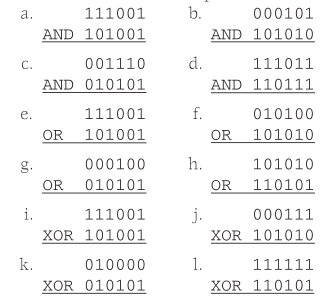
\includegraphics[scale = 0.7]{images/P34.png}
  
  \Answer 

  \begin{tabular}{l r     l r}
    a. &     111001 & b. &     000101 \\
       & AND 101001 &    & AND 101010 \\ \cline{2-2} \cline{4-4}
       &     101001 &    &     000000 \\
       &            &    &            \\
    c. &     001110 & d. &     111011 \\
       & AND 010101 &    & AND 110111 \\ \cline{2-2} \cline{4-4}
       &     000100 &    &     110011 \\
       &            &    &            \\
    e. &     111001 & f. &     010100 \\
       & OR  101001 &    & OR  101010 \\ \cline{2-2} \cline{4-4}
       &     111001 &    &     111110 \\
       &            &    &            \\
    g. &     000100 & h. &     101010 \\
       & OR  010101 &    & OR  110101 \\ \cline{2-2} \cline{4-4}
       &     010101 &    &     111111 \\
       &            &    &            \\
    i. &     111001 & j. &     000111 \\
       & XOR 101001 &    & XOR 101010 \\ \cline{2-2} \cline{4-4}
       &     010000 &    &     101101 \\
       &            &    &            \\
    k. &     010000 & h. &     111111 \\
       & XOR 010101 &    & XOR 110101 \\ \cline{2-2} \cline{4-4}
       &     000101 &    &     001010 \\
       &            &    &            \\
    
  \end{tabular}
  
\end{homeworkProblem}


\begin{homeworkProblem}[Problem 41]
  Write a program in the machine language of Appendix C that reverses the contents of the memory cell at address 8C. (That is, the final bit pattern at address 8C when read from left to right should agree with the original pattern when read from right to left.)
  
  \Answer 
  %% 0 src
  %% 1 dst
  %% A 1 (to perform AND) 
  %% B the result of AND

\begin{verbatim}
108C
2100
2A01
8BA0
A001
A107
711B
8BA0
A001
A107
711B
8BA0
A001
A107
711B
8BA0
A001
A107
711B
8BA0
A001
A107
711B
8BA0
A001
A107
711B
8BA0
A001
A107
711B
8BA0
A001
A107
711B
318C
C000
\end{verbatim}
  
\end{homeworkProblem}


% \Acknowledgement{Thank XXX XX 2004010102 and XXX XXXX 2004010103 for the discussion about ...}

% End edit to here
%%%%%%%%%%%%%%%%%%%%%%%%%%%%%%%%%%%%%%%%%%%%%%%%%%%%%%%%%%%%%

\end{spacing}
\end{document}

%%%%%%%%%%%%%%%%%%%%%%%%%%%%%%%%%%%%%%%%%%%%%%%%%%%%%%%%%%%%%
